% Generated by code/scripts/report_figures.py at 2026-10-30T09:20:59Z; do not edit.
% Inputs: artifacts/local/runs/pipeline-e2e-20261030T092022Z/run
\begin{figure}[t]
\centering
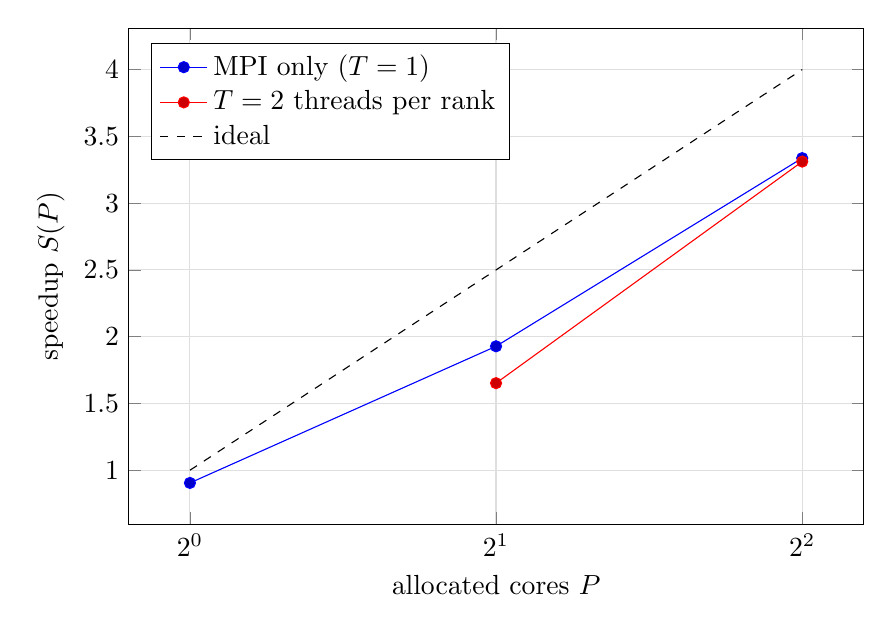
\begin{tikzpicture}
\begin{axis}[width=0.9\columnwidth, height=0.65\columnwidth, xlabel={allocated cores $P$}, ylabel={speedup $S(P)$}, xmode=log, log basis x=2, legend pos=north west, legend cell align=left, grid=major, grid style={gray!25}]
\addplot+[mark=*] coordinates {(1,0.905) (2,1.928) (4,3.337)};
\addlegendentry{MPI only ($T=1$)}
\addplot+[mark=*] coordinates {(2,1.652) (4,3.311)};
\addlegendentry{$T=2$ threads per rank}
\addplot[black, dashed] coordinates {(1,1) (4,4)};
\addlegendentry{ideal}
\end{axis}
\end{tikzpicture}
\caption{\textbf{LOCAL PIPELINE TEST, NOT A MEASUREMENT.} Strong-scaling speedup. $N=4000$, median of repetitions; serial Barnes--Hut baseline on the same CPU model and build.}
\label{fig:strong-speedup}
\end{figure}
